\documentclass[a4paper]{article}

\usepackage[english]{babel}
\usepackage[utf8]{inputenc}
\usepackage{amsmath}
\usepackage{graphicx}
\usepackage[colorinlistoftodos]{todonotes}
\usepackage{enumerate}
\usepackage{eqnarray}

\textheight=10in
\textwidth=6.9in
\topmargin=0.0in
\headheight=-0.3in
\headsep=-0.3in
\leftmargin=-0.2in
\rightmargin=-0.4in
\oddsidemargin=-0.3in
\evensidemargin=-0.5in
\parindent=0.0in

\pagestyle{empty}

\def\ss{\displaystyle\sum}
\def\ii{\displaystyle\int}
\def\lb{\left(}
\def\rb{\right)}
\def\lB{\left[}
\def\rB{\right]}
\def\E{\mathrm{E}}
\def\Var{\mathrm{Var}}
\def\Cov{\mathrm{Cov}}
\def\Pr{\mathrm{Pr}}
\def\erf{\mathrm{erf}}
\def\erfinv{\mathrm{erfinv}}
\linespread{1.2}

\title{FINA4140 HW4}

\author{You}

\date{\today}

\begin{document}
\begin{enumerate}
\item Problem 1\\
Refer to Q1.m\\
Input: interest rate, initial stock price, time to maturity, strike price, observed option price, number of steps to be carried out by the program\\
Then, the method is similar to ch14, except:\\
When we calculate the increment, we use the calculated value of call/put and the true value depending on the type of option specified by the user;\\
The number of steps does not depend on whether the change in sigma in each step. Instead, it only depends on the input by the user.



\pagebreak

\item Problem 2
\begin{enumerate}
\item
The error $=\frac{z_{0.025}s_n}{\sqrt{n}}$, where $z_{0.025}\approx 1.96$, $s_n$ is the sample standard deviation of $e^z$ and $n$ is the sample size.\\
Since $\sigma=\sqrt{(e-1)e}\approx 2.16$, $s_n$ should be close to this.\\
Set $\frac{z_{0.025}s_n}{\sqrt{n}}=10^{-4},n=1.96^2(e-1)e(10^8)$\\
Hence, if the error has to be in the order of -4, the sample size $n$ has to be in the order of 8.\\
Similarly, if the error has to be in the order of -6, the sample size $n=1.96^2(e-1)e(10^{12})$, which is in the order of 12.\\
For Fig. 15.2,  the error $=\frac{z_{0.025}s_n}{\sqrt{n}}$, and now $s_n$ is the sample standard deviation of $S_T$\\
Assuming $S_t=S_0\exp\lb\lb r-\frac{1}{2}\sigma^2\rb t+\sigma\sqrt{t}Z\rb$\\
$\Var(S_T)=\lb e^{\sigma^2T}-1\rb\lb e^{2(r-\sigma^2/2)T+\sigma^2T}\rb$\\
Therefore, to reduce the error to $10^{-6}$,\\
the number of samples required $=1.96^2\lb e^{\sigma^2T}-1\rb\lb e^{2(r-\sigma^2/2)T+\sigma^2T}\rb 10^{12}$

\pagebreak

\item
Using $2^5,2^6,\cdots,2^{17}$ samples, we repeatedly run the algorithm in ch15 to obtain point estimate and confidence interval.\\
For the case of call, the option value in each simulation is $e^{-rT}\max(S-E,0)$\\
For the case of put, the option value in each simulation is $e^{-rT}\max(E-S,0)$\\
Then, we can plot a grpah of the point estimate and confidence interval against number of samples.\\
Also, we use the program ch08 from Problem 1 to obtain the analytical value of the option and plot a horizontal line of the analytical value on the same graph.\\
Running the program Q2bCall.m and Q2bPut.m, we obtain the following graphs:
\begin{figure}[ht]
\centering
\includegraphics[width=0.5\textwidth]{Q2b.png}
\caption{\label{fig:fig01a} Monte-Carlo approximations to a European Call value}
\end{figure}

\begin{figure}[ht]
\centering
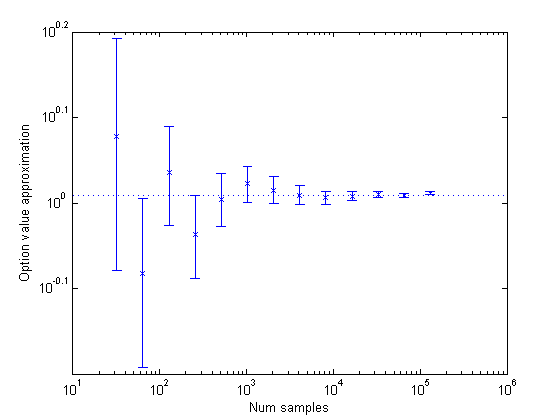
\includegraphics[width=0.5\textwidth]{Q2bPut.png}
\caption{\label{fig:fig01b} Monte-Carlo approximations to a European Put value}
\end{figure}


\end{enumerate}

\pagebreak

\item Problem 3
\begin{enumerate}
\item 
For $X$ and $Y$ being independent random variables from the same distribution, it is always true that $(f(X)-f(Y))(g(X)-g(Y))\geq 0$\\
Therefore, the expected value of $(f(X)-f(Y))(g(X)-g(Y))$ is non-negative.\\
$\E\left[(f(X)-f(Y))(g(X)-g(Y))\right]\geq 0\\
\E\left[f(X)g(X)\right]-\E\left[f(Y)g(X)\right]-\E\left[f(X)g(Y)\right]+\E\left[f(Y)g(Y)\right]\geq 0\\
2\E\left[f(X)g(X)\right]-2\E\left[f(X)\right]\E\left[g(X)\right]\geq 0\\
\E\left[f(X)g(X)\right]\geq\E\left[f(X)\right]\E\left[g(X)\right]$


\item
Assume $g$ is a monotonic increasing function on $X_1,\cdots,X_n$, then it is also increasing on $U_1,\cdots,U_n$ as the cumulative distribution function is increasing.\\
Hence, $Y$ is increasing on $U_1,\cdots,U_n$ and $Y'$ is decreasing on $U_1,\cdots,U_n$\\
Since $Y$ and $-Y'$ are increasing on $U_1,\cdots,U_n$, by the results of (a), we have $\E\left[-YY'\right]\geq\E\left[Y\right]\E\left[-Y'\right]$\\
So, $\E\left[YY'\right]\leq\E\left[Y\right]\E\left[Y'\right]$ and $\Cov(Y,Y')\leq 0$\\
Therefore, $Y$ and $Y'$ are negatively correlated.

\end{enumerate}

\pagebreak

\item Problem 4
\begin{enumerate}
\item
Input: Initial stock price S, interest rate r, volatility $\sigma$, strike price K, time to maturity T, number of simulations of payoff N\\
Output: Pmean is the computed price, conf is the 95\% confidence interval.\\
$Z =$ Vector with N independent $U(0,1)$ samples\\
The simulated stock price and antithetic value are generated to be $Se^{r-0.5\sigma^2}T\pm\sigma\sqrt{T}Z$ respectively.\\
Value of option = Arithmetic mean of $(e^{-rT}\max(S_\text{simulated}-K,0))$\\
Obtaining the sample mean and variance of sample for the stock price, the calculated price is the sample mean, while the confidence interval is $\left[X-1.96\sqrt{\frac{V}{N}},X+1.96\sqrt{\frac{V}{N}} \right]$


\item
Using the method in 4(a), we can obtain the value of the options. We also use the code in ch10 to find the analytical values.\\
Calculating the absolute error, we can find that the value calculated from Monte Carlo method converges to the analytical value as number of MC steps increases, but the effect is not uniform. The effect fluctuates between increase and decrease in absolute error but eventually absolute error converges to 0.\\

\begin{table}[ht]
	\centering
    \begin{tabular}{|l|l|l|l|l|l|l|}
    \hline
    T                         & 0.5     & 1       & 0.5    & 1       & 0.5     & 1       \\ \hline
    K                         & 80      & 80      & 100    & 100     & 120     & 120     \\ \hline
    Analytical Value for Call & 21.8351 & 24.1472 & 7.7603 & 11.3485 & 1.7669  & 4.4633  \\ \hline
    Computed Price for Call   & 21.8686 & 24.1400 & 7.7241 & 11.3401 & 1.7674  & 4.4128  \\ \hline
    Analytical Value for Put  & 0.6440  & 1.7828  & 6.2715 & 8.3930  & 19.9803 & 20.9168 \\ \hline
    Computed Price for Put    & 0.6576  & 1.7814  & 6.2451 & 8.3877  & 19.9817 & 20.8946 \\ \hline
    \end{tabular}
\end{table}

In the graph below, graphs in first row: T=0.5; second row: T=1\\
graphs in first column: K=80; second column: K=100; third column: K=120
\begin{figure}[ht]
\centering
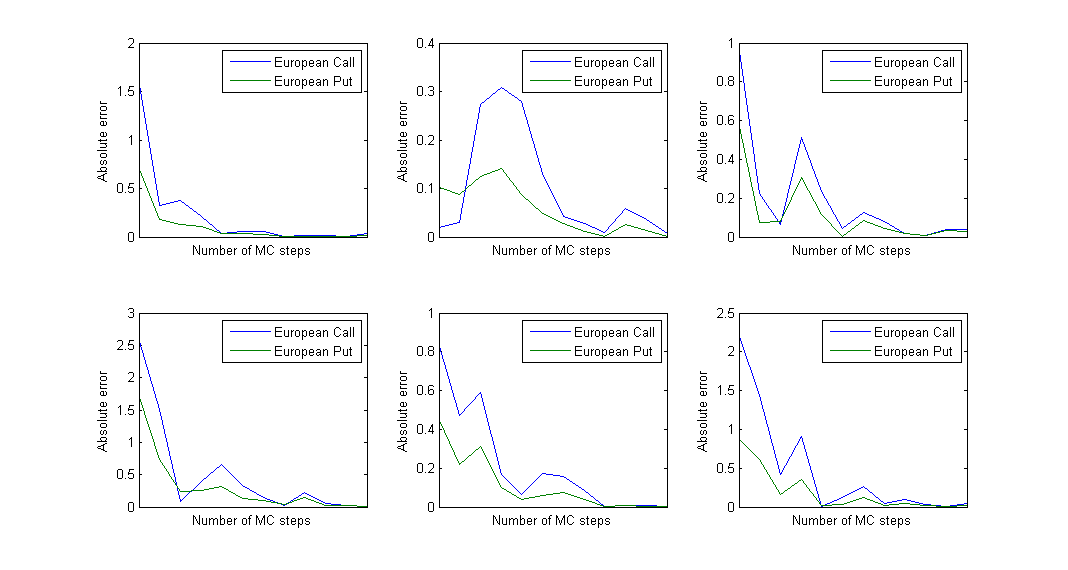
\includegraphics[width=0.7\textwidth]{Q4b.png}
\caption{\label{fig:fig02} MC approximation of values of European Call and Put}
\end{figure}

\pagebreak

\item
The method is the same as in 4(b), except that the value of the option is calculated by\\ $e^{-rT}\max(0,S(t)^n-k^n)$. The conclusions on convergence behavior are the same as in 4(b); as n increases, the absolute error when number of MC steps is small increases (it still converges to 0 as MC steps increases).\\

\begin{table}[ht]
	\centering
    \begin{tabular}{|l|l|l|l|l|l|l|}
    \hline
    T                                          & 0.5    & 1      & 0.5    & 1      & 0.5    & 1      \\ \hline
    K                                          & 80     & 80     & 100    & 100    & 120    & 120    \\ \hline
    Analytical Value for n=2 ($\times10^3$)    & 4.2660 & 5.0096 & 1.7564 & 2.7335 & 0.4669 & 1.2290 \\ \hline
    Computed Price for n=2 ($\times10^3$)      & 4.2638 & 5.0242 & 1.7767 & 2.7308 & 0.4670 & 1.2511 \\ \hline
    Analytical Value for n=3 ($\times10^5$)    & 6.3812 & 8.0889 & 3.0238 & 5.0617 & 0.9061 & 2.6222 \\ \hline
    Computed Price for n=3 ($\times10^5$)      & 6.3717 & 8.1221 & 3.0253 & 5.0696 & 0.9031 & 2.5837 \\ \hline
    Analytical Value for n=4 ($\times10^8$)    & 0.8686 & 1.2200 & 0.4673 & 0.8550 & 0.1613 & 0.4924 \\ \hline
    Computed Price for n=4 ($\times10^8$)      & 0.8709 & 1.2202 & 0.4671 & 0.8547 & 0.1619 & 0.5042 \\ \hline
    Analytical Value for n=5 ($\times10^{10}$) & 1.1362 & 1.8134 & 0.6840 & 1.4040 & 0.2696 & 0.9131 \\ \hline
    Computed Price for n=5 ($\times10^{10}$)   & 1.1408 & 1.8071 & 0.6897 & 1.3935 & 0.2712 & 0.9227 \\ \hline
    \end{tabular}
\end{table}

In the graph below, graphs in the 1st row: n=2; 2nd row: n=3; 3rd row: n=4; 4th row: n=5\\
graphs in columns 1,3,5: T=0.5;  columns 2,4,6: T=1\\
graphs in columns 1,2: K=80; columns 3,4: K=100; columns 5,6: K=120
\begin{figure}[ht]
\centering
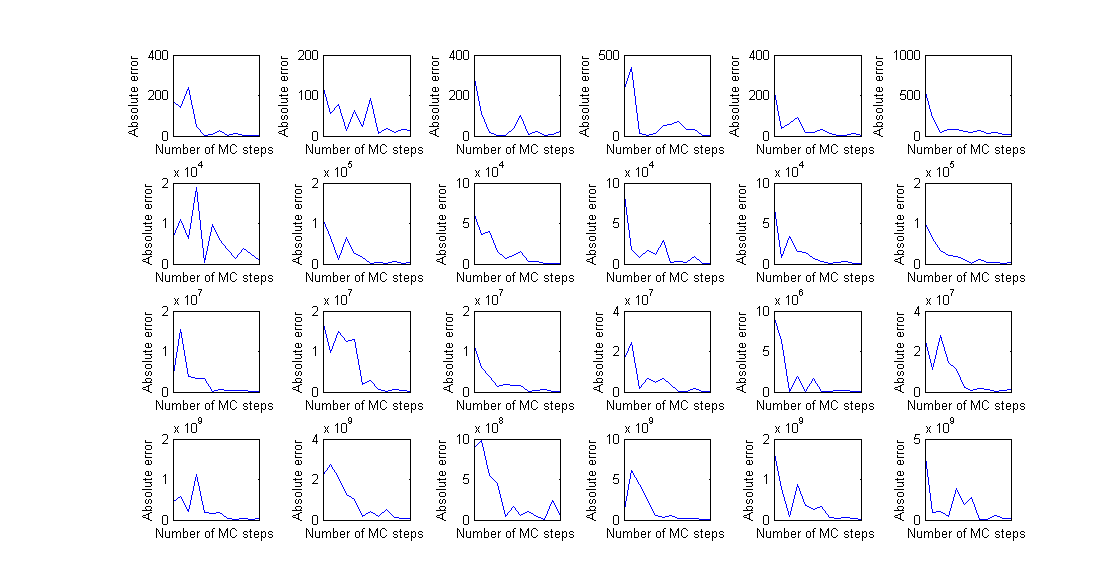
\includegraphics[width=0.7\textwidth]{Q4c.png}
\caption{\label{fig:fig03} MC approximation of values of Asymmetric Power Call}
\end{figure}

\pagebreak

\item
The method is the same as in 4(b), except that the value of the option is calculated by $e^{-rT}|S(T)-K|$. The conclusions on convergence behavior are the same as in 4(b).\\
The analytical value is calculated by the sum of the analytical values of a European call and European put with same parameters as the straddle.\\

\begin{table}[ht]
	\centering
    \begin{tabular}{|l|l|l|l|l|l|l|}
    \hline
    T                             & 0.5     & 1       & 0.5     & 1       & 0.5     & 1       \\ \hline
    K                             & 80      & 80      & 100     & 100     & 120     & 120     \\ \hline
    Analytical Value for Straddle & 22.4791 & 25.9300 & 14.0317 & 19.7415 & 21.7472 & 25.3801 \\ \hline
    Computed Price for Straddle   & 22.6179 & 25.9381 & 13.9874 & 19.7378 & 21.6593 & 25.2921 \\ \hline
    \end{tabular}
\end{table}

In the graph below, graphs in first row: T=0.5; second row: T=1\\
graphs in first column: K=80; second column: K=100; third column: K=120
\begin{figure}[ht]
\centering
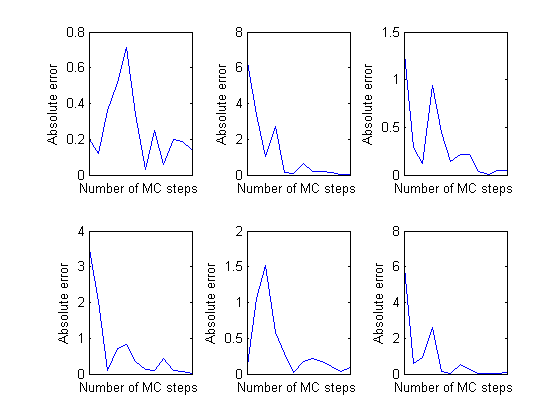
\includegraphics[width=0.7\textwidth]{Q4d.png}
\caption{\label{fig:fig04} MC approximation of values of straddle}
\end{figure}

\end{enumerate}

\pagebreak

\item Problem 5\\
The parts changed from program ch24 are:\\
The lower bound of the stock price is the barrier instead of 0, since the option is worthless if stock price is lower than the barrier. Since the number of different stock prices (i.e. variable Nx) is unchanged, the value of h is adjusted.\\
The payoff at maturity becomes that of a call, i.e. $\max(S-E,0)$.\\
The variables bca and bcb, which reflect the boundary conditions, are changed to those of a call option.\\
The label for z-axis of the graph is changed to “Down-and-out call value”.\\
Calculations of p and q are changed as follows:\\
Apply FTCS with $F=(1-rk)I+\frac{1}{2}k\sigma^2\hat{D_2}T_2+\frac{1}{2}kr\hat{D_1}T_1$, where
\[\hat{D_1}=\begin{bmatrix}  
\frac{B+h}{h} & 0 & \cdots & \cdots & 0\\
0 & \frac{B+2h}{h} & 0 & \ddots & \vdots\\
0 & 0 & \frac{B+3h}{h} & \ddots & \vdots\\
\vdots & \ddots & \ddots & \ddots & 0\\
0 & \cdots & \cdots & 0 & \frac{B+(N_x-1)h}{h}
\end{bmatrix}
\]
and $\hat{D_2}=\hat{D_1}^2$, with
\[
p^i=\begin{bmatrix}
\lb k\frac{1}{2}\sigma^2\frac{(B+h)^2}{h^2}-rk\frac{(B+h)}{2h}\rb V_0^i\\
0\\
\vdots\\
0\\
\lb k\frac{1}{2}\sigma^2\frac{(B+(N_x-1)h)^2}{h^2}-rk\frac{(B+(N_x-1)h)}{2h}\rb V_{N_x}^i
\end{bmatrix}
\]
Similarly, apply BTCS with $B=(1+rk)I-\frac{1}{2}k\sigma^2\hat{D_2}T_2-\frac{1}{2}kr\hat{D_1}T_1$ and
\[
q^i=\begin{bmatrix}
\lb k\frac{1}{2}\sigma^2\frac{(B+h)^2}{h^2}-rk\frac{(B+h)}{2h}\rb V_0^{i+1}\\
0\\
\vdots\\
0\\
\lb k\frac{1}{2}\sigma^2\frac{(B+(N_x-1)h)^2}{h^2}-rk\frac{(B+(N_x-1)h)}{2h}\rb V_{N_x}^{i+1}
\end{bmatrix}
\]
Running the program Q5.m, we obtain the following graph:
\begin{figure}[ht]
\centering
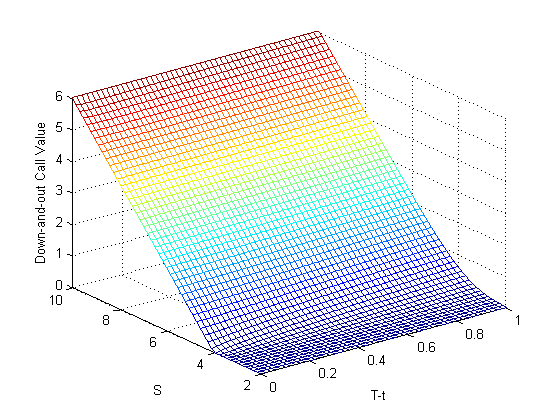
\includegraphics[width=0.5\textwidth]{Q5.png}
\caption{\label{fig:fig05} Down-and-Out Call value at different T-t and S}
\end{figure}

\end{enumerate}
\end{document}